
\begin{figure}[]{}
    \centering
	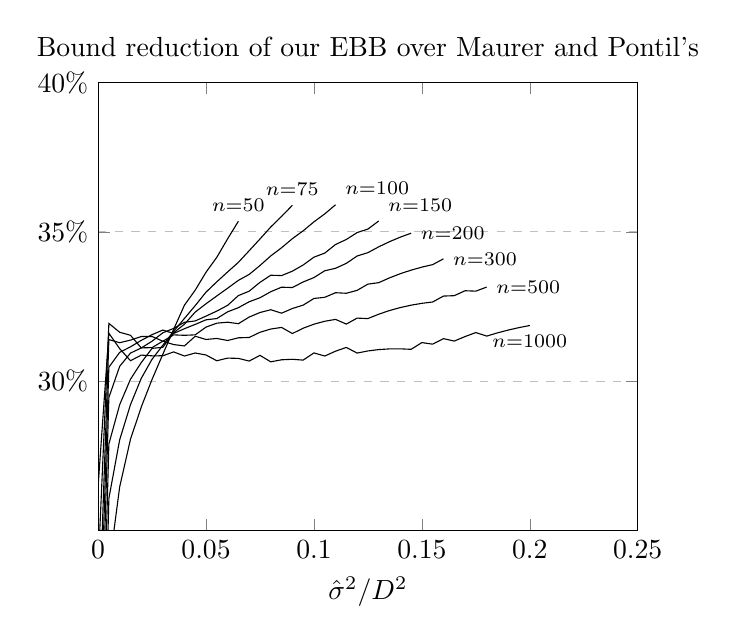
\begin{tikzpicture}
	\begin{axis}[
		title={Bound reduction of our EBB over  Maurer and Pontil's},
		xlabel={$\hat{\sigma}^2/D^2$},
		xmin=0, xmax=0.25,
		ymin=25, ymax=40,
		xtick={0,0.05,0.1,0.15,0.2,0.25},
		ytick={30,35,40},
		yticklabel=$\pgfmathprintnumber{\tick}\%$,
		ymajorgrids=true,
		grid style=dashed,
		xticklabel style={/pgf/number format/fixed},
	]
	\addplot[] coordinates {
(0.0, 10.038489469957923)(0.005, 23.729228874038338)(0.01, 26.46795119155083)(0.015, 28.061119743643296)(0.02, 29.141938583623652)(0.025, 30.066155991693723)(0.03, 30.907282335052788)(0.035, 31.738722848538305)(0.04, 32.54914392836502)(0.045, 33.05291848928947)(0.05, 33.651509619741496)(0.055, 34.151805087746446)(0.06, 34.768247610158575)(0.065, 35.35764746719292)
		}node[pos=1.0](endofplotsquare){} ;
	\node [above] at (endofplotsquare) {$\scriptstyle n=50$};
	\addplot[] coordinates {
(0.0, 12.591458904845746)(0.005, 26.08582516018055)(0.01, 28.044488963240152)(0.015, 29.219014176778845)(0.02, 30.101019545112305)(0.025, 30.739739304373572)(0.03, 31.209391146592484)(0.035, 31.67459564986504)(0.04, 32.10560417423678)(0.045, 32.53522214247566)(0.05, 32.98480753922602)(0.055, 33.33123349968554)(0.06, 33.66064263107598)(0.065, 33.983296057116895)(0.07, 34.371432119724126)(0.075, 34.76400092304011)(0.08, 35.165771922230526)(0.085, 35.51929445366766)(0.09, 35.890640326573575)
		}node[pos=1.0](endofplotsquare){} ;
	\node [above] at (endofplotsquare) {$\scriptstyle n=75$};
	\addplot[] coordinates {
(0.0, 14.817995440815901)(0.005, 27.90751007185735)(0.01, 29.219819451516923)(0.015, 30.070639062533996)(0.02, 30.629290720122317)(0.025, 31.104197838170627)(0.03, 31.14038996461402)(0.035, 31.62526607199946)(0.04, 31.911575841232846)(0.045, 32.3187069670152)(0.05, 32.59698646227685)(0.055, 32.85814963311234)(0.06, 33.115830685662)(0.065, 33.379908028841236)(0.07, 33.578110917203176)(0.075, 33.87653264786374)(0.08, 34.19803078792182)(0.085, 34.470564003329045)(0.09, 34.774201537103245)(0.095, 35.03784322660741)(0.1, 35.337583634279)(0.105, 35.60362789769355)(0.11, 35.90890662248758)
		}node[pos=1.0](endofplotsquare){} ;
	\node [above right] at (endofplotsquare) {$\scriptstyle n=100$};
	\addplot[] coordinates {
(0.0, 17.342661445161745)(0.005, 29.461247776997926)(0.01, 30.502124709956824)(0.015, 30.94634600450878)(0.02, 31.116833768989828)(0.025, 31.344627574353588)(0.03, 31.62499327739429)(0.035, 31.772139980592)(0.04, 31.975727165299386)(0.045, 32.02196228998142)(0.05, 32.183034431467235)(0.055, 32.352369659168474)(0.06, 32.54250416890406)(0.065, 32.87047963677422)(0.07, 33.017679271803296)(0.075, 33.31333732160584)(0.08, 33.55087101615144)(0.085, 33.53938459819124)(0.09, 33.68714872653657)(0.095, 33.89275583281304)(0.1, 34.15600891069251)(0.105, 34.290920495879966)(0.11, 34.57974857223946)(0.115, 34.747357884723435)(0.12, 34.97811379083637)(0.125, 35.09584827017029)(0.13, 35.36531839253051)
		}node[pos=1.0](endofplotsquare){} ;
	\node [above right] at (endofplotsquare) {$\scriptstyle n=150$};
	\addplot[] coordinates {
(0.0, 19.269181617386778)(0.005, 30.47328215171227)(0.01, 30.970505248952783)(0.015, 31.155076903228505)(0.02, 31.370737591330126)(0.025, 31.563153411429678)(0.03, 31.716924278688328)(0.035, 31.602163041853583)(0.04, 31.762160711176872)(0.045, 31.905759719654245)(0.05, 32.05956774531062)(0.055, 32.101874254626836)(0.06, 32.32639539364612)(0.065, 32.465858041087344)(0.07, 32.663895247621326)(0.075, 32.797586647322234)(0.08, 32.99998541625402)(0.085, 33.15092115439265)(0.09, 33.13907818080335)(0.095, 33.32527974281349)(0.1, 33.47347491095124)(0.105, 33.70030345616673)(0.11, 33.78337094262078)(0.115, 33.94866206353597)(0.12, 34.19406008169977)(0.125, 34.30666804274627)(0.13, 34.5014054670121)(0.135, 34.67351335871075)(0.14, 34.82497129829329)(0.145, 34.95753413863828)
		}node[pos=1.0](endofplotsquare){} ;
	\node [right] at (endofplotsquare) {$\scriptstyle n=200$};
	\addplot[] coordinates {
(0.0, 21.01455983414305)(0.005, 31.398323351742654)(0.01, 31.29316800287044)(0.015, 31.380044700971307)(0.02, 31.499573558604126)(0.025, 31.501955199548522)(0.03, 31.342388805161228)(0.035, 31.555898653589576)(0.04, 31.540720961712708)(0.045, 31.556719994430246)(0.05, 31.815518124296712)(0.055, 31.947447662218103)(0.06, 31.979020008525413)(0.065, 31.929950573976118)(0.07, 32.151946530365926)(0.075, 32.30372613153442)(0.08, 32.39631985663968)(0.085, 32.28147349936643)(0.09, 32.43775937546441)(0.095, 32.55064623256504)(0.1, 32.77372870056995)(0.105, 32.81284419609248)(0.11, 32.96572615770543)(0.115, 32.94748952790814)(0.12, 33.04474761150041)(0.125, 33.25359991684834)(0.13, 33.30204392434083)(0.135, 33.462830030160355)(0.14, 33.601886363972085)(0.145, 33.7211101175424)(0.15, 33.822185822075845)(0.155, 33.90661477833436)(0.16, 34.09961256888578)
		}node[pos=1.0](endofplotsquare){} ;
	\node [right] at (endofplotsquare) {$\scriptstyle n=300$};
	\addplot[] coordinates {
(0.0, 23.733576061543907)(0.005, 31.93999128292596)(0.01, 31.642400396531094)(0.015, 31.54212092349261)(0.02, 31.12052542652318)(0.025, 31.129819611252405)(0.03, 31.344098301521242)(0.035, 31.231838999520004)(0.04, 31.185453514912005)(0.045, 31.51029078782499)(0.05, 31.401697787018254)(0.055, 31.43592520457107)(0.06, 31.367624957687056)(0.065, 31.45753767654653)(0.07, 31.468778394474676)(0.075, 31.6423499409508)(0.08, 31.751037287923307)(0.085, 31.804794091938522)(0.09, 31.59991862434968)(0.095, 31.778311022724473)(0.1, 31.913384999263183)(0.105, 32.010501900631745)(0.11, 32.074189915872516)(0.115, 31.915973789453584)(0.12, 32.11613625130849)(0.125, 32.10053700848796)(0.13, 32.24708311545571)(0.135, 32.3692691037866)(0.14, 32.46936498795406)(0.145, 32.54937215145163)(0.15, 32.61106237732128)(0.155, 32.65601018366708)(0.16, 32.85390573088976)(0.165, 32.867317678660584)(0.17, 33.03199624865481)(0.175, 33.01872182909822)(0.18, 33.15487119563348)
		}node[pos=1.0](endofplotsquare){} ;
	\node [right] at (endofplotsquare) {$\scriptstyle n=500$};
	\addplot[] coordinates {
(0.0, 26.48466951022569)(0.005, 31.610541001763814)(0.01, 31.094245131329373)(0.015, 30.691021818068354)(0.02, 30.878933354114203)(0.025, 30.854623560301786)(0.03, 30.855718952687877)(0.035, 30.985476785778605)(0.04, 30.84839664811395)(0.045, 30.94907807084863)(0.05, 30.882232292715344)(0.055, 30.68950445827823)(0.06, 30.77857995587979)(0.065, 30.768677505684852)(0.07, 30.679146150855704)(0.075, 30.870441770906094)(0.08, 30.653781659199446)(0.085, 30.72198559607093)(0.09, 30.738566645167236)(0.095, 30.710992728150178)(0.1, 30.95229310334558)(0.105, 30.847606478652455)(0.11, 31.009527688997892)(0.115, 31.135832380489546)(0.12, 30.946326663430018)(0.125, 31.017664917855072)(0.13, 31.06348584444511)(0.135, 31.08638415275851)(0.14, 31.0886271157673)(0.145, 31.072204850949028)(0.15, 31.29715291414822)(0.155, 31.244828197450204)(0.16, 31.429852460842593)(0.165, 31.347766957340134)(0.17, 31.49894525891586)(0.175, 31.63356906325342)(0.18, 31.514234978296805)(0.185, 31.62214364046394)(0.19, 31.716729481001114)(0.195, 31.79891328121711)(0.2, 31.869534804168858)
		}node[pos=1.0](endofplotsquare){} ;
	\node [below] at (endofplotsquare) {$\scriptstyle n=1000$};
	\end{axis}
	\end{tikzpicture}
	\vspace{-10pt}
	\caption[The percent reduction our EBB would achieve]{The percent reduction of the 0.5 probability bound, that going from Maurer and Pontil's EBB to our EBB would achieve, for various $n$, in the domain valid for their EBB.}
	\label{biggraph3}
	
	
	\vspace{15pt}
	
	
	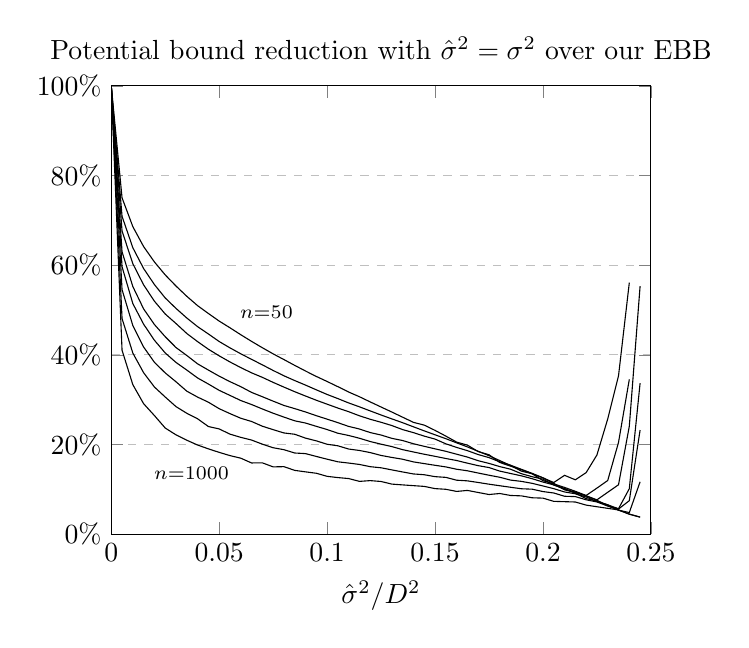
\begin{tikzpicture}
	\begin{axis}[
		title={Potential bound reduction with $\hat{\sigma}^2 = \sigma^2$ over our EBB},
		xlabel={$\hat{\sigma}^2/D^2$},
		xmin=0, xmax=0.25,
		ymin=0, ymax=100,
		xtick={0,0.05,0.1,0.15,0.2,0.25},
		ytick={0,20,40,60,80,100},
		yticklabel=$\pgfmathprintnumber{\tick}\%$,
		legend pos=south west,
		ymajorgrids=true,
		grid style=dashed,
		xticklabel style={/pgf/number format/fixed},
	]
	\addplot[] coordinates {
(0.0, 100.0)(0.005, 75.02420135527589)(0.01, 68.58202038924931)(0.015, 64.13237924865832)(0.02, 60.71118820468343)(0.025, 57.819103972950124)(0.03, 55.33498759305211)(0.035, 53.04630381803412)(0.04, 50.96)(0.045, 49.21383647798742)(0.05, 47.51937984496124)(0.055, 46.02446483180428)(0.06, 44.47806354009077)(0.065, 42.99625468164794)(0.07, 41.57386785449146)(0.075, 40.20618556701031)(0.08, 38.93352812271731)(0.085, 37.63596809282088)(0.09, 36.38328530259366)(0.095, 35.17191977077364)(0.1, 34.04558404558404)(0.105, 32.88447909284196)(0.11, 31.68666196189132)(0.115, 30.639494026704146)(0.12, 29.481792717086833)(0.125, 28.35195530726257)(0.13, 27.228412256267408)(0.135, 26.0778859527121)(0.14, 24.930555555555557)(0.145, 24.31129476584022)(0.15, 23.140495867768596)(0.155, 21.862068965517242)(0.16, 20.525224602626125)(0.165, 19.8489010989011)(0.17, 18.413793103448278)(0.175, 17.707618393960193)(0.18, 15.975103734439834)(0.185, 15.161957270847692)(0.19, 14.36426116838488)(0.195, 13.452299245024022)(0.2, 12.542837559972584)(0.205, 11.51473612063057)(0.21, 13.115845539280958)(0.215, 12.117177097203728)(0.22, 13.71280724450194)(0.225, 17.65424557116677)(0.23, 25.69558101472995)(0.235, 35.30794546309356)(0.24, 56.085994309200125)
		}node[pos=0.4](endofplotsquare){} ;
	\node [above right] at (endofplotsquare) {$\scriptstyle n=50$};
	\addplot[] coordinates {
(0.0, 100.0)(0.005, 70.89337175792507)(0.01, 63.881401617250674)(0.015, 59.23076923076923)(0.02, 55.66502463054187)(0.025, 52.67538644470868)(0.03, 50.345622119815665)(0.035, 48.20627802690583)(0.04, 46.2800875273523)(0.045, 44.646680942184155)(0.05, 42.96218487394958)(0.055, 41.54639175257732)(0.06, 40.22289766970618)(0.065, 38.983050847457626)(0.07, 37.75811209439528)(0.075, 36.50485436893204)(0.08, 35.31669865642994)(0.085, 34.25047438330171)(0.09, 33.23943661971831)(0.095, 32.18604651162791)(0.1, 31.152073732718893)(0.105, 30.228310502283104)(0.11, 29.257246376811594)(0.115, 28.39173405211141)(0.12, 27.475468331846567)(0.125, 26.572187776793623)(0.13, 25.704225352112676)(0.135, 24.84689413823272)(0.14, 23.93385552654482)(0.145, 23.03030303030303)(0.15, 22.155172413793103)(0.155, 21.28755364806867)(0.16, 20.35928143712575)(0.165, 19.453924914675767)(0.17, 18.46808510638298)(0.175, 17.502124044180118)(0.18, 16.397621070518266)(0.185, 15.306122448979592)(0.19, 14.054514480408859)(0.195, 13.463166807790008)(0.2, 11.925042589437819)(0.205, 11.205432937181664)(0.21, 10.414902624894157)(0.215, 9.551986475063398)(0.22, 8.622147083685546)(0.225, 10.262725779967159)(0.23, 11.961722488038278)(0.235, 20.45616535994298)(0.24, 34.51481696687972)
		}node[pos=0.693](endofplotsquare){} ;
	%\node [above] at (endofplotsquare) {$\scriptstyle n=75$};
	\addplot[] coordinates {
(0.0, 100.0)(0.005, 67.61904761904762)(0.01, 60.31468531468531)(0.015, 55.5921052631579)(0.02, 51.95618153364632)(0.025, 49.0990990990991)(0.03, 46.97406340057637)(0.035, 44.75524475524475)(0.04, 42.93478260869565)(0.045, 41.246684350132625)(0.05, 39.766839378238345)(0.055, 38.40304182509506)(0.06, 37.142857142857146)(0.065, 35.97560975609756)(0.07, 34.97005988023952)(0.075, 33.844339622641506)(0.08, 32.7906976744186)(0.085, 31.76605504587156)(0.09, 30.804077010192525)(0.095, 29.86577181208054)(0.1, 28.98230088495575)(0.105, 28.11816192560175)(0.11, 27.302275189599133)(0.115, 26.394849785407725)(0.12, 25.61105207226355)(0.125, 24.94736842105263)(0.13, 24.217118997912316)(0.135, 23.316062176165804)(0.14, 22.633744855967077)(0.145, 21.859039836567927)(0.15, 21.196754563894523)(0.155, 20.141700404858298)(0.16, 19.335347432024168)(0.165, 18.61861861861862)(0.17, 17.74675972083749)(0.175, 17.063492063492063)(0.18, 16.12265084075173)(0.185, 15.369458128078819)(0.19, 14.454277286135694)(0.195, 13.555992141453832)(0.2, 12.561334641805692)(0.205, 11.307767944936087)(0.21, 9.881422924901186)(0.215, 9.251968503937007)(0.22, 8.537782139352306)(0.225, 7.647058823529412)(0.23, 9.333333333333334)(0.235, 11.00832562442183)(0.24, 24.0625)(0.245, 55.32786885245902)
		}node[pos=1.0](endofplotsquare){} ;
	%\node [above] at (endofplotsquare) {$n=100$};
	\addplot[] coordinates {
(0.0, 100.0)(0.005, 62.98342541436464)(0.01, 55.223880597014926)(0.015, 50.23041474654378)(0.02, 46.753246753246756)(0.025, 44.03292181069959)(0.03, 41.61735700197239)(0.035, 39.84819734345351)(0.04, 37.981651376146786)(0.045, 36.58969804618117)(0.05, 35.233160621761655)(0.055, 34.00673400673401)(0.06, 32.89473684210526)(0.065, 31.612903225806452)(0.07, 30.647709320695103)(0.075, 29.658385093167702)(0.08, 28.702290076335878)(0.085, 27.994011976047904)(0.09, 27.245949926362297)(0.095, 26.41509433962264)(0.1, 25.644699140401148)(0.105, 24.858757062146893)(0.11, 24.022346368715084)(0.115, 23.448275862068964)(0.12, 22.646657571623464)(0.125, 22.10242587601078)(0.13, 21.36181575433912)(0.135, 20.871862615587848)(0.14, 20.157068062827225)(0.145, 19.58495460440986)(0.15, 19.02313624678663)(0.155, 18.471337579617835)(0.16, 17.825537294563844)(0.165, 17.189460476787954)(0.17, 16.375)(0.175, 15.77639751552795)(0.18, 15.061728395061728)(0.185, 14.478527607361963)(0.19, 13.480392156862745)(0.195, 12.804878048780488)(0.2, 12.257281553398059)(0.205, 10.94890510948905)(0.21, 10.194174757281553)(0.215, 9.101941747572816)(0.22, 7.907542579075426)(0.225, 7.38498789346247)(0.23, 6.521739130434782)(0.235, 5.669481302774427)(0.24, 10.136674259681094)(0.245, 33.693843594009984)
		}node[pos=1.0](endofplotsquare){} ;
	%\node [above] at (endofplotsquare) {$n=150$};
	\addplot[] coordinates {
(0.0, 100.0)(0.005, 59.642857142857146)(0.01, 51.41955835962145)(0.015, 46.820809248554916)(0.02, 43.24324324324324)(0.025, 40.40920716112532)(0.03, 38.292682926829265)(0.035, 36.5967365967366)(0.04, 34.831460674157306)(0.045, 33.47826086956522)(0.05, 32.06751054852321)(0.055, 30.942622950819672)(0.06, 29.8)(0.065, 28.90625)(0.07, 27.915869980879542)(0.075, 26.96629213483146)(0.08, 26.102941176470587)(0.085, 25.270758122743683)(0.09, 24.778761061946902)(0.095, 24.041811846689896)(0.1, 23.32761578044597)(0.105, 22.504230118443317)(0.11, 22.0)(0.115, 21.38157894736842)(0.12, 20.650406504065042)(0.125, 20.064205457463885)(0.13, 19.523809523809526)(0.135, 18.838304552590266)(0.14, 18.322981366459626)(0.145, 17.81874039938556)(0.15, 17.35159817351598)(0.155, 16.867469879518072)(0.16, 16.417910447761194)(0.165, 15.828402366863905)(0.17, 15.27165932452276)(0.175, 14.847161572052402)(0.18, 14.057971014492754)(0.185, 13.525179856115107)(0.19, 13.0)(0.195, 12.357954545454545)(0.2, 11.614730878186968)(0.205, 10.985915492957746)(0.21, 10.0)(0.215, 9.396914446002805)(0.22, 8.531468531468532)(0.225, 7.5524475524475525)(0.23, 6.3113604488078545)(0.235, 5.594405594405594)(0.24, 7.462686567164179)(0.245, 23.214285714285715)
		}node[pos=1.0](endofplotsquare){} ;
	%\node [above] at (endofplotsquare) {$n=200$};
	\addplot[] coordinates {
(0.0, 100.0)(0.005, 54.54545454545455)(0.01, 46.52173913043478)(0.015, 41.732283464566926)(0.02, 38.32116788321168)(0.025, 35.95890410958904)(0.03, 33.980582524271846)(0.035, 31.888544891640866)(0.04, 30.56379821958457)(0.045, 29.428571428571427)(0.05, 27.977839335180054)(0.055, 26.881720430107528)(0.06, 25.848563968668408)(0.065, 25.126903553299492)(0.07, 24.069478908188586)(0.075, 23.300970873786408)(0.08, 22.565320665083135)(0.085, 22.273781902552205)(0.09, 21.4123006833713)(0.095, 20.80536912751678)(0.1, 20.044052863436125)(0.105, 19.696969696969695)(0.11, 18.976545842217483)(0.115, 18.658280922431867)(0.12, 18.181818181818183)(0.125, 17.551020408163264)(0.13, 17.10261569416499)(0.135, 16.69980119284294)(0.14, 16.110019646365423)(0.145, 15.728155339805825)(0.15, 15.355086372360844)(0.155, 14.990512333965844)(0.16, 14.473684210526315)(0.165, 14.12639405204461)(0.17, 13.627992633517495)(0.175, 13.138686131386862)(0.18, 12.681159420289855)(0.185, 12.050359712230216)(0.19, 11.764705882352942)(0.195, 11.327433628318584)(0.2, 10.73943661971831)(0.205, 10.13986013986014)(0.21, 9.40766550522648)(0.215, 8.996539792387543)(0.22, 8.290155440414507)(0.225, 7.253886010362694)(0.23, 6.540447504302926)(0.235, 5.344827586206897)(0.24, 4.810996563573883)(0.245, 11.67192429022082)
		}node[pos=1.0](endofplotsquare){} ;
	%\node [above] at (endofplotsquare) {$n=300$};
	\addplot[] coordinates {
(0.0, 100.0)(0.005, 48.091603053435115)(0.01, 40.38461538461539)(0.015, 36.0)(0.02, 32.8125)(0.025, 30.58252427184466)(0.03, 28.440366972477065)(0.035, 26.956521739130434)(0.04, 25.726141078838175)(0.045, 24.0)(0.05, 23.46153846153846)(0.055, 22.304832713754646)(0.06, 21.58273381294964)(0.065, 20.97902097902098)(0.07, 20.068027210884352)(0.075, 19.269102990033222)(0.08, 18.83116883116883)(0.085, 18.095238095238095)(0.09, 17.956656346749227)(0.095, 17.325227963525837)(0.1, 16.71641791044776)(0.105, 16.129032258064516)(0.11, 15.85014409221902)(0.115, 15.536723163841808)(0.12, 15.041782729805014)(0.125, 14.794520547945206)(0.13, 14.324324324324325)(0.135, 13.866666666666667)(0.14, 13.421052631578947)(0.145, 13.246753246753247)(0.15, 12.820512820512821)(0.155, 12.658227848101266)(0.16, 12.030075187969924)(0.165, 11.881188118811881)(0.17, 11.519607843137255)(0.175, 11.138014527845037)(0.18, 10.79136690647482)(0.185, 10.451306413301662)(0.19, 10.117647058823529)(0.195, 10.023310023310023)(0.2, 9.49074074074074)(0.205, 9.174311926605505)(0.21, 8.447488584474886)(0.215, 8.371040723981901)(0.22, 7.657657657657658)(0.225, 7.174887892376682)(0.23, 6.263982102908278)(0.235, 5.369127516778524)(0.24, 4.464285714285714)(0.245, 3.7861915367483294)
		}node[pos=1.0](endofplotsquare){} ;
	%\node [above] at (endofplotsquare) {$n=500$};
	\addplot[] coordinates {
(0.0, 100.0)(0.005, 41.02564102564103)(0.01, 33.333333333333336)(0.015, 29.09090909090909)(0.02, 26.446280991735538)(0.025, 23.66412213740458)(0.03, 22.142857142857142)(0.035, 20.945945945945947)(0.04, 19.871794871794872)(0.045, 19.01840490797546)(0.05, 18.235294117647058)(0.055, 17.51412429378531)(0.06, 16.939890710382514)(0.065, 15.873015873015873)(0.07, 15.897435897435898)(0.075, 15.0)(0.08, 15.048543689320388)(0.085, 14.218009478672986)(0.09, 13.88888888888889)(0.095, 13.574660633484163)(0.1, 12.88888888888889)(0.105, 12.608695652173912)(0.11, 12.393162393162394)(0.115, 11.764705882352942)(0.12, 11.934156378600823)(0.125, 11.740890688259109)(0.13, 11.155378486055778)(0.135, 10.980392156862745)(0.14, 10.81081081081081)(0.145, 10.64638783269962)(0.15, 10.150375939849624)(0.155, 10.0)(0.16, 9.523809523809524)(0.165, 9.747292418772563)(0.17, 9.285714285714286)(0.175, 8.8339222614841)(0.18, 9.059233449477352)(0.185, 8.620689655172415)(0.19, 8.532423208191126)(0.195, 8.108108108108109)(0.2, 8.02675585284281)(0.205, 7.308970099667774)(0.21, 7.2368421052631575)(0.215, 7.166123778501628)(0.22, 6.472491909385114)(0.225, 6.109324758842444)(0.23, 5.7507987220447285)(0.235, 5.396825396825397)(0.24, 4.444444444444445)(0.245, 3.7974683544303796)
		}node[pos=0.85](endofplotsquare){} ;
	\node [below left] at (endofplotsquare) {$\scriptstyle n=1000$};
	\end{axis}
	\end{tikzpicture}
	\vspace{-10pt}
	\caption[The percent reduction our EBB could yet achieve]{The percent reduction in the 0.5 probability bound that going from our EBB to using Bennett's inequality (perfect variance information, $\hat{\sigma}^2 = \sigma^2$) achieves, for $n=50,75,100,150,200,300,500,1000$.}
	\label{biggraph4}
\end{figure}
